\documentclass{article}

\usepackage{graphicx}
\usepackage[utf8]{inputenc}

\title{Exabiome Journal}
\author{kellyhuang }
\date{August 2020}

\begin{document}

\maketitle

\section{VGG Experiments }
VGG11 after a run of 200 epochs produced an accuracy of 73.94\% on the small dataset (about 22\% worse than using Roznet) and an accuracy of 47.85\% on the medium dataset. VGG13 gave an even worse accuracy score of 43.32\%. VGG16 and VGG19 produced errors so they were not included. 


\subsubsection*{Small dataset: 200 epochs per run}
\begin{figure}[h!]
  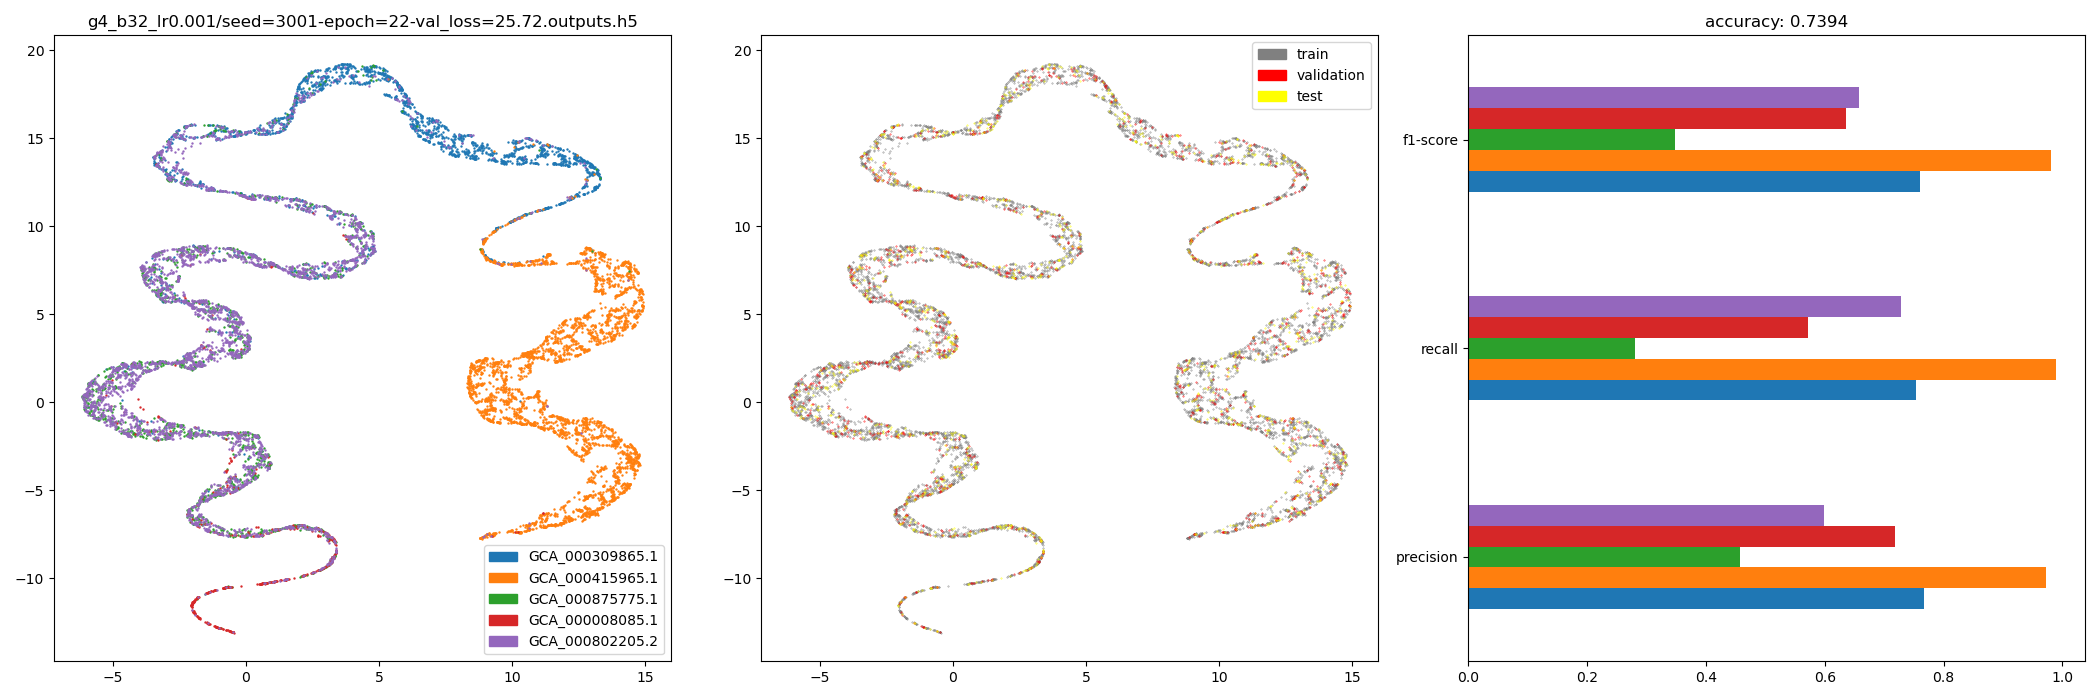
\includegraphics[width=\linewidth]{new_journal/figures/experiments/vgg/small/vgg11/run1.png}
  \caption{VGG11 Run 1}
\end{figure}

\begin{figure}[h!]
  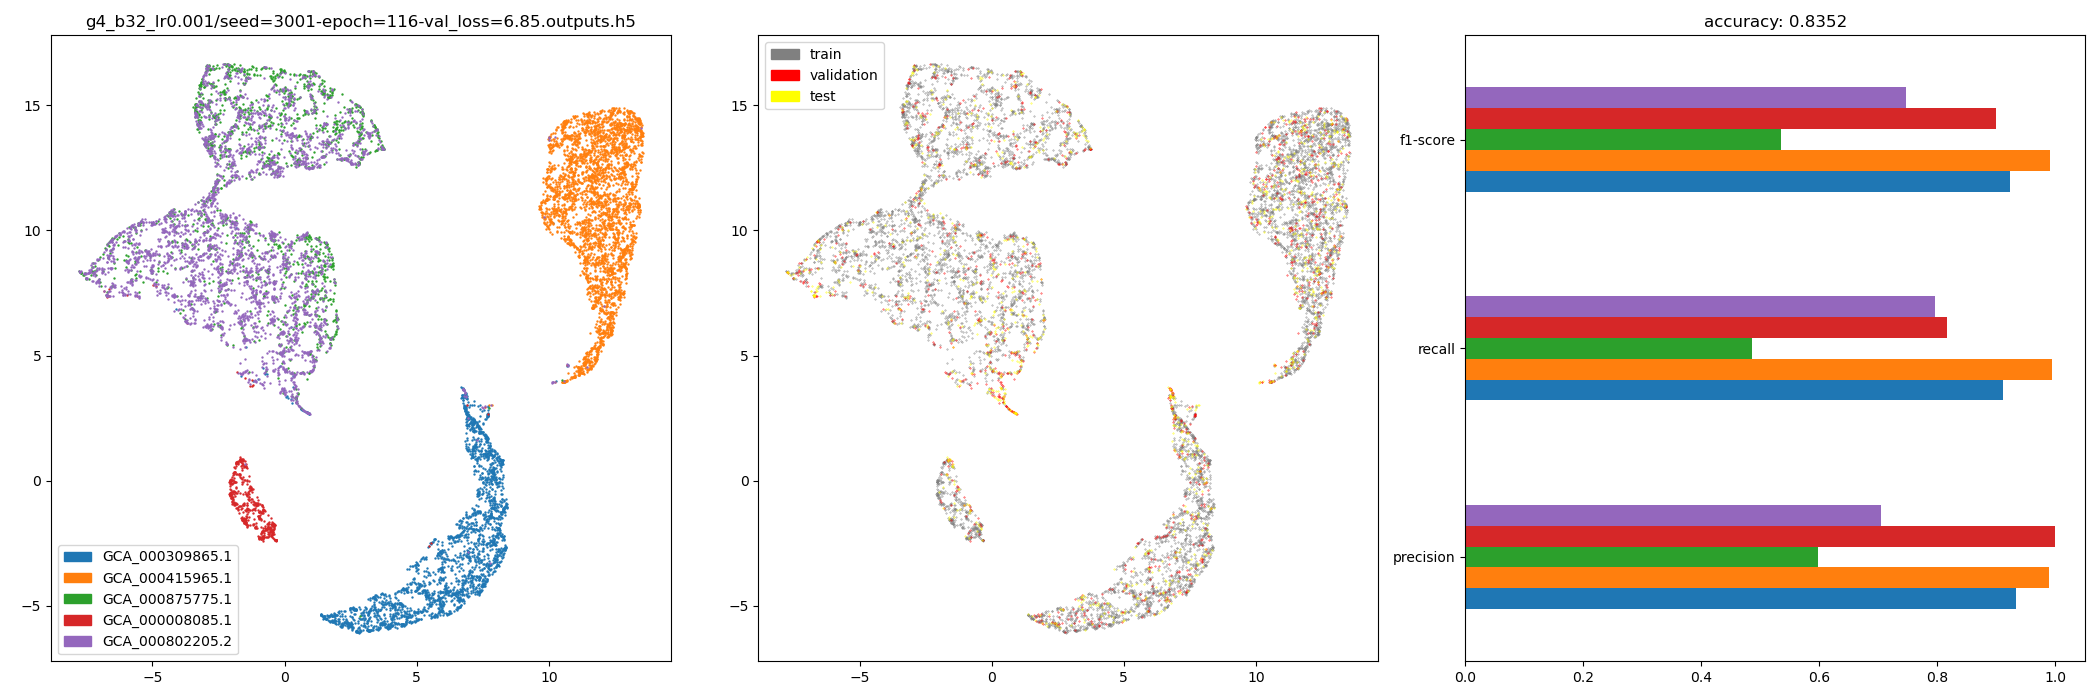
\includegraphics[width=\linewidth]{new_journal/figures/experiments/vgg/small/vgg11/run2.png}
  \caption{VGG11 Run 2}
\end{figure}

\clearpage

\subsubsection*{Medium dataset}
\begin{figure}[h!]
  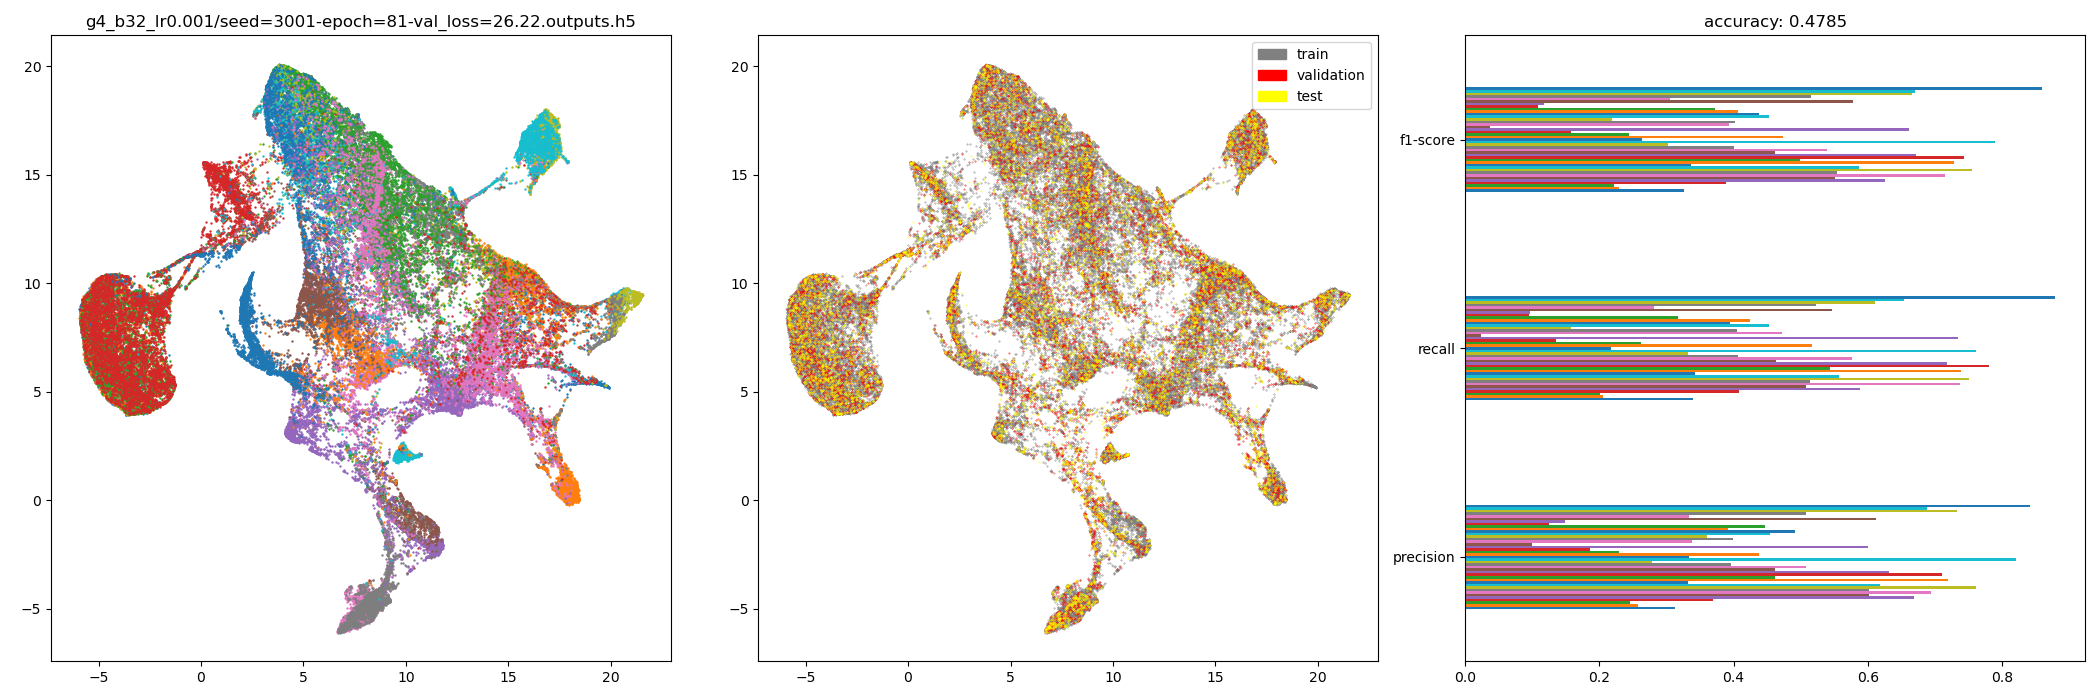
\includegraphics[width=\linewidth]{new_journal/figures/experiments/vgg/medium/vgg11/seed=3001-epoch=81-val_loss=26.22.outputs.png}
  \caption{VGG11 Run 1}
\end{figure}

\begin{figure}[h!]
  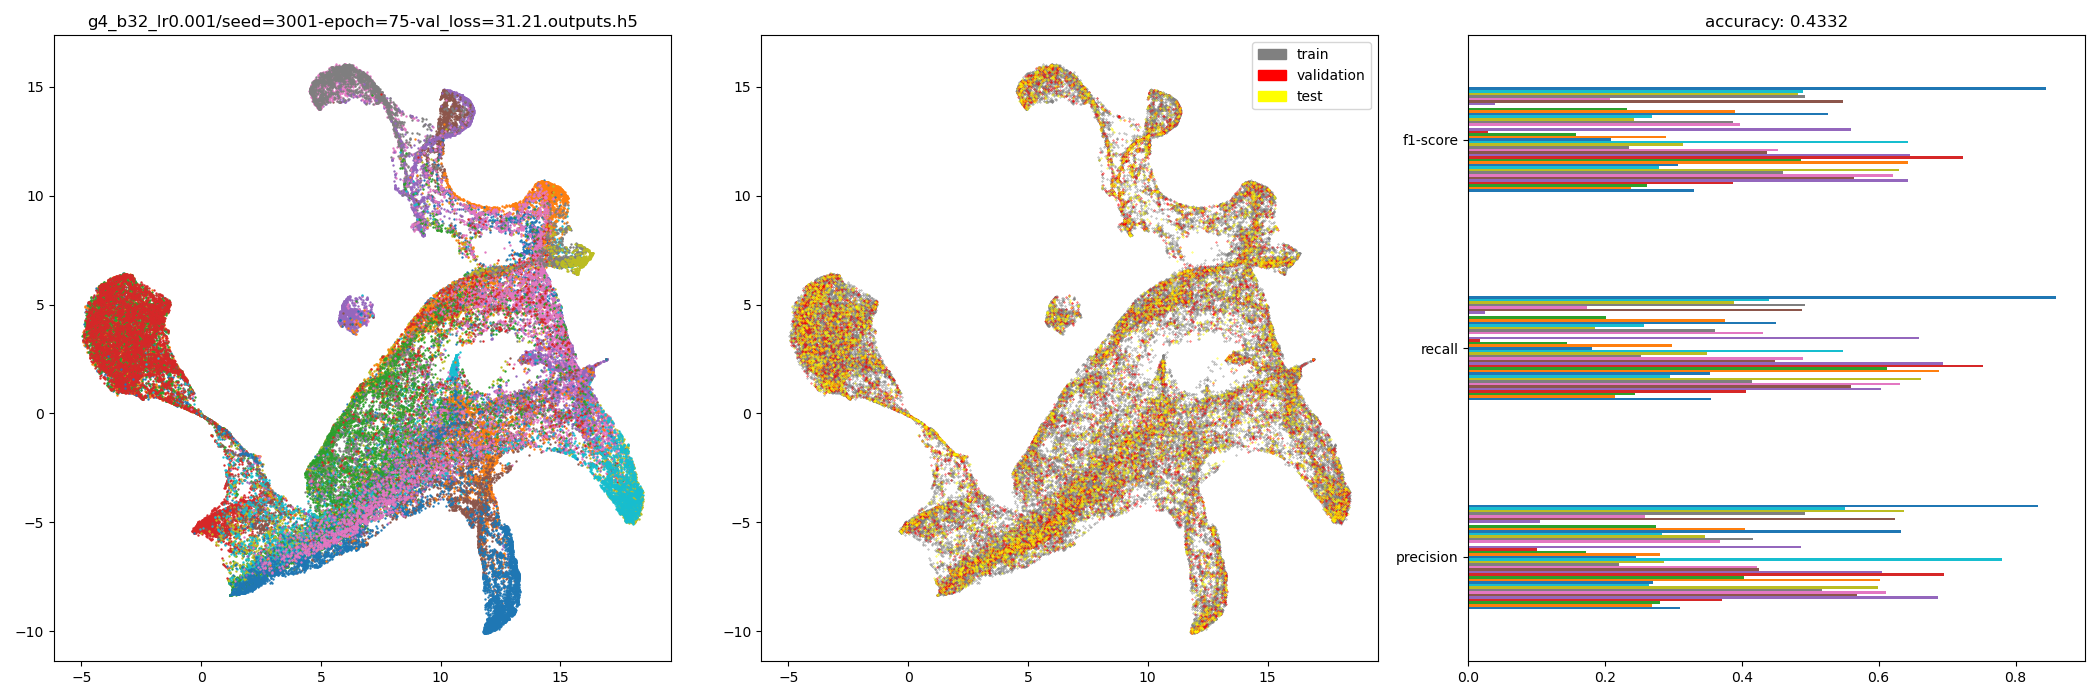
\includegraphics[width=\linewidth]{new_journal/figures/experiments/vgg/medium/vgg13/seed=3001-epoch=75-val_loss=31.21.outputs.png}
  \caption{VGG13 Run 1}
\end{figure}

\end{document}


